\renewcommand{\theequation}{\theenumi}
\begin{enumerate}[label=\thesubsection.\arabic*.,ref=\thesubsection.\theenumi]
\numberwithin{equation}{enumi}
\item 
Find the point at which the tangent to the curve 
%\cite{twelve_one}
\begin{align}
y = \sqrt{4x-3}-1
\label{eq:parab}
\end{align}
has slope $\frac{2}{3}$.
\\
\solution \eqref{eq:parab} can be expressed as
\begin{align}
\brak{y+1}^2 &= 4x-3
\\
\text{or, } y^2  -4x + 2y+ 4 &= 0
\label{eq:parab_twovar}
\end{align}
which has the form \eqref{eq:conic_quad_form} with parameters
\begin{align}
\vec{V} = \myvec{0 & 0\\0 & 1}, \vec{u} = \myvec{-2\\1}, f = 4.
\label{eq:parab_twovar_params}
\end{align}
Thus, the given curve is a parabola.  $\because \vec{V}$ is diagonal and in standard form,
\begin{align}
\vec{P} = \vec{I} \implies \vec{p}_1 = \myvec{1\\0}
\label{eq:parab_ex1_eig}
\end{align}
From Table \ref{table:conics}, the 
focus is 4
and the vertex $\vec{c}$ is
\begin{align}
\myvec{ -4 & 1 \\ 0 & 0 \\ 0 & 1}\vec{c} &= \myvec{-4 \\ 0\\-1} 
\\
\implies 
\myvec{ -4 & 1 \\  0 & 1}\vec{c} &= \myvec{-4 \\ -1} 
\\
\text{or, } \vec{c} = \myvec{\frac{3}{4}\\-1}
\end{align}
The direction vector and normal vectors are
\begin{align}
\vec{m} = \myvec{1 \\ \frac{2}{3}} = \myvec{3\\2}, \vec{n} = \myvec{2\\-3}.
\label{eq:parab_twovar_mn}
\end{align}
Also, 
\begin{align}
\vec{V}\vec{p} &= \vec{0}
\\
\implies \vec{p} &= \myvec{1\\0}
\label{eq:parab_twovar_p}
\end{align}
From \eqref{eq:conic_tangent_qk_eigen}, \eqref{eq:parab_twovar_mn} and \eqref{eq:parab_twovar_p},
\begin{align}
\kappa = -1
\end{align}
which, upon substitution in \eqref{eq:conic_tangent_q_eigen} and simplification yields the matrix equation
\begin{align}
\myvec{-4 & 4\\0 & 0\\0&1}\vec{q} &= \myvec{-4\\0\\2}
\\
\implies \myvec{-4 & 4\\0&1}\vec{q} &= \myvec{-4\\2}
\\
\text{or, } \vec{q} &= \myvec{3\\2}
\end{align}
Fig. \ref{fig:parab_tangent}	verifies the above results.
%
\begin{figure}[!ht]
\centering
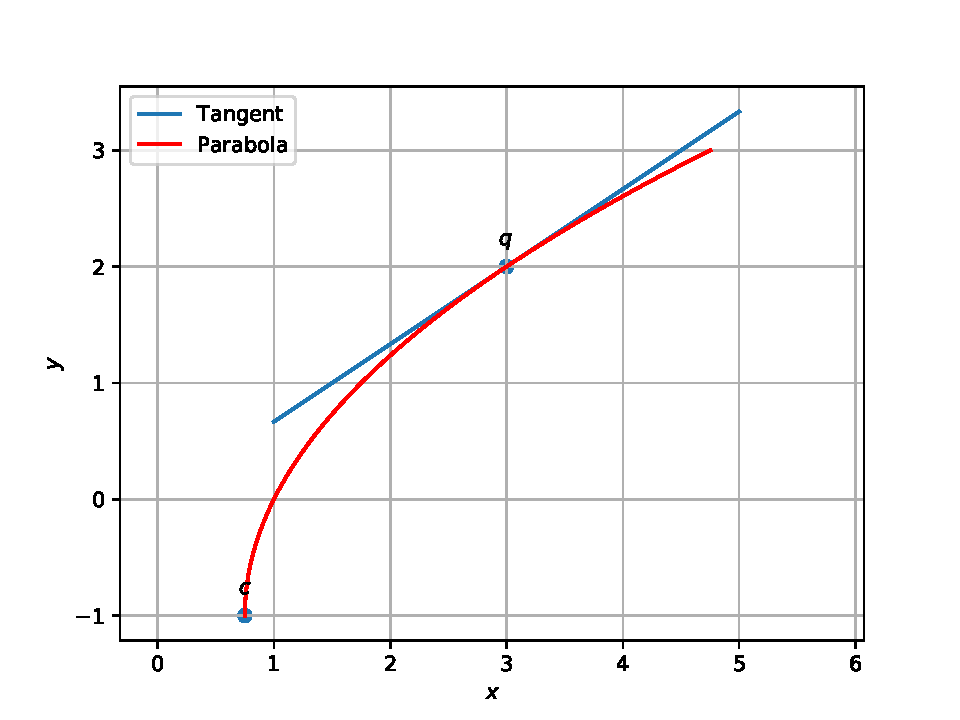
\includegraphics[width=\columnwidth]{./figs/parab/parab_tangent.eps}
\caption{Tangent to  parabola in \eqref{eq:parab}  with slope $\frac{2}{3}$. }
\label{fig:parab_tangent}	
\end{figure}

\item 
Find a point on the curve 
%\cite{twelve_one}
\begin{align}
y = \brak{x-2}^2
\label{eq:parab_secant}
\end{align}
at which the tangent is parallel to the chord joining the points (2, 0) and (4, 4).
\\
\solution \eqref{eq:parab_secant} can be expressed as
\begin{align}
x^2  -4x - y + 4 &= 0
\label{eq:parab_secant_twovar}
\end{align}
which has the form \eqref{eq:conic_quad_form} with parameters
\begin{align}
\vec{V} = \myvec{1 & 0\\0 & 0},  \vec{u} = -\myvec{2\\\frac{1}{2}}, f = 4.
\label{eq:parab_secant_twovar_params}
\end{align}
Using eigenvalue decomposition, 
\begin{align}
\vec{P} = \myvec{0 & 1\\1 & 0}, \vec{D} = \myvec{0 & 0\\0 & 1}
\end{align}
%
Hence, the eigenvector of $\vec{V}$ corresponding to the zero eigenvalue is
\begin{align}
\vec{p}_1 = \myvec{0\\1}.
\end{align}
Substituting the above parameters in the equation for the vertex of the parabola in Table \ref{table:conics},
\begin{align}
\myvec{-2 & -\frac{5}{2} \\ 1 & 0 \\ 0 & 0}\vec{c} &= \myvec{-4 \\ 2 \\ 0}
\\
\implies \myvec{-1 & -\frac{5}{2} \\ 1 & 0}\vec{c} &= \myvec{-4 \\ 2 }
\\
\text{or, } \vec{c} &= \myvec{2\\0}
\end{align}
The direction vector is
\begin{align}
\vec{m} = \myvec{4 \\ 4}-\myvec{2 \\ 0} = \myvec{1\\2}
\label{eq:parab_secant_twovar_m}
\end{align}
and normal vector is
\begin{align}
\vec{n} =  \myvec{2\\-1}
\label{eq:parab_secant_twovar_n}
\end{align}
From the equation for the point of contact for the  parabola  in Table \ref{table:conics},
%\eqref{eq:conic_tangent_qk_eigen}, \eqref{eq:parab_secant_twovar_params}
% and \eqref{eq:parab_secant_twovar_n} 
\begin{align}
\kappa = \frac{1}{2}
\end{align}
resulting in the matrix equation
\begin{align}
\myvec{-1 & -1\\1 & 0\\0&0}\vec{q} &= \myvec{-4\\3\\0}
\\
\implies \myvec{-1 & -1\\1 & 0}\vec{q} &= \myvec{-4\\3}
\\
\text{or, } \vec{q} &= \myvec{3\\1}
\end{align}
Fig. \ref{fig:parab_secant_tangent}	verifies the above results.  Note that $\vec{P}$ rotates the standard parabola by 90\degree.
%
\begin{figure}[!ht]
\centering
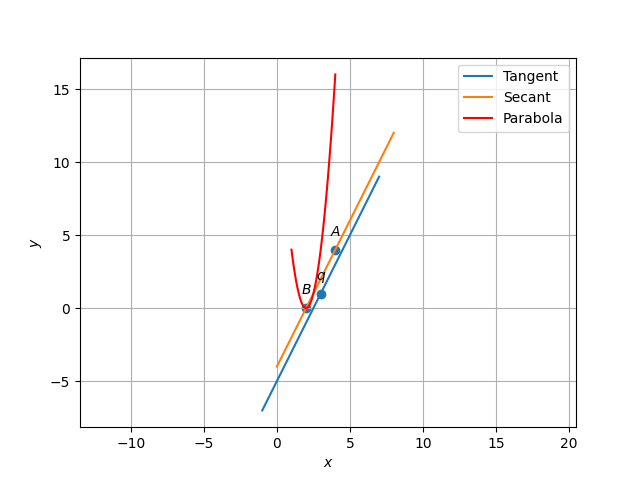
\includegraphics[width=\columnwidth]{./figs/parab/parab_tangent_secant.eps}
\caption{Tangent to  parabola in \eqref{eq:parab_secant}  is parallel to the line joining the points \myvec{2\\ 0} and \myvec{4\\ 4}. }
\label{fig:parab_secant_tangent}	
\end{figure}
%
\item What conic does the following equation represent. 
\begin{align}
9x^2-24xy+16y^2-18x-101y+19 = 0
\label{eq:conics/ex/solution/given}
\end{align}
Find the center.
%
\\
\solution
From theory, we understand that using dot product we can find the angle between the lines 
\begin{enumerate}
	\item 
	\begin{align}\label{eq:solutions/line_plane/74/codes:5}
		\frac{x-2}{2} = \frac{y-1}{5} &= \frac{z+3}{-3}, 
	\end{align}
	\begin{align}\label{eq:solutions/line_plane/74/codes:6}
		\frac{x+2}{-1} = \frac{y-4}{8} &= \frac{z-5}{4} 
	\end{align}


The above symmetric equations \ref{eq:solutions/line_plane/74/codes:5}, \ref{eq:solutions/line_plane/74/codes:6} can be represented in the vector form as 
\begin{align}\label{eq:solutions/line_plane/74/codes7}
	\quad \vec{r_1} &= \myvec{2\\1\\-3} + \lambda_1\myvec{2\\5\\-3}
	\\
	\quad \vec{r_2} &= \myvec{-2\\4\\5} + \lambda_2\myvec{-1\\8\\4}
\end{align}

As we have to find the angle between the vectors, we will only be taking the direction vectors into consideration. The direction vectors are $\vec{u}$ = $\myvec{2\\5\\-3}$ and $\vec{v}$ = $\myvec{-1\\8\\4}$. We can find the corresponding magnitude values

\begin{align}\label{eq:solutions/line_plane/74/codes9}
	\norm{\vec{u}} =\sqrt{2^{2}+5^{2}+(-3)^{2}} =\sqrt{38}
\end{align}
\begin{align}\label{eq:solutions/line_plane/74/codes10}
	\norm{\vec{v}} =\sqrt{(-1)^{2}+8^{2}+4^{2}} =\sqrt{81}
\end{align}

Using \ref{eq:solutions/line_plane/74/codes4}, \ref{eq:solutions/line_plane/74/codes9}, \ref{eq:solutions/line_plane/74/codes10} we get
\begin{align}
	\theta = \cos ^{-1}\frac{\myvec{2\\5\\-3}^{T}\myvec{-1\\8\\4}}{(\sqrt{38})(\sqrt{81})} 
	\\
	\theta = \cos ^{-1}\frac{26}{55.4797}
	\\
	\theta = \cos ^{-1} (0.4686)
	\\
	\theta = 62.053\degree
\end{align}

Therefore, the angle between the two lines is $62.053\degree$.See Fig. \ref{fig:solutions/line_plane/74/codesline_equation_1}

\begin{figure}
	\centering
	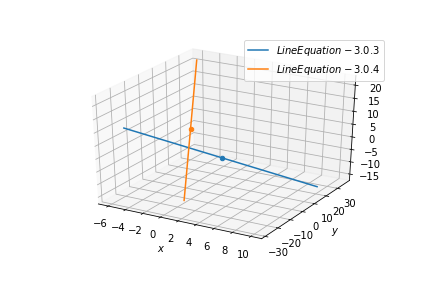
\includegraphics[width=\columnwidth]{./solutions/line_plane/74/codes/figs/Line_interest_1.png}
	\caption{Graph for equations \ref{eq:solutions/line_plane/74/codes7}}
	\label{fig:solutions/line_plane/74/codesline_equation_1}
\end{figure}


	\item 
	\begin{align}\label{eq:solutions/line_plane/74/codes12}
		\frac{x}{2} = \frac{y}{2} &= \frac{z}{1}, 
	\end{align}
	\begin{align}\label{eq:solutions/line_plane/74/codes13}
		\frac{x-5}{4} = \frac{y-2}{1} &= \frac{z-3}{8} 
	\end{align}



The above symmetric equations \ref{eq:solutions/line_plane/74/codes12}, \ref{eq:solutions/line_plane/74/codes13} can be represented in the vector form as 
\begin{align}\label{eq:solutions/line_plane/74/codes14}
	\quad \vec{r_1} &= \myvec{0\\0\\0} + \lambda_1\myvec{2\\2\\1}
	\\
	\quad \vec{r_2} &= \myvec{5\\2\\3} + \lambda_2\myvec{4\\1\\8}
\end{align}

As we have to find the angle between the vectors, we will only be taking the direction vectors into consideration. The direction vectors are $\vec{u}$ = $\myvec{2\\2\\1}$ and $\vec{v}$ = $\myvec{4\\1\\8}$. We can find the corresponding magnitude values

\begin{align}\label{eq:solutions/line_plane/74/codes16}
	\norm{\vec{u}} =\sqrt{2^{2}+2^{2}+1^{2}} =\sqrt{9}
\end{align}
\begin{align}\label{eq:solutions/line_plane/74/codes17}
	\norm{\vec{v}} =\sqrt{4^{2}+1^{2}+8^{2}} =\sqrt{81}
\end{align}

Using \ref{eq:solutions/line_plane/74/codes4}, \ref{eq:solutions/line_plane/74/codes16}, \ref{eq:solutions/line_plane/74/codes17} we get
\begin{align}
	\theta = \cos ^{-1}\frac{\myvec{2\\2\\1}^{T}\myvec{4\\1\\8}}{(\sqrt{9})(\sqrt{81})} 
	\\
	\theta = \cos ^{-1}\frac{18}{27.00}
	\\
	\theta = \cos ^{-1} (0.667)
	\\
	\theta = 48.189\degree
\end{align}

Therefore, the angle between the two lines is $48.189\degree$. See Fig. \ref{fig:solutions/line_plane/74/codesline_equation_2}


\begin{figure}
	\centering
	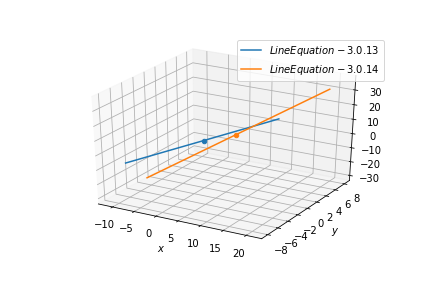
\includegraphics[width=\columnwidth]{./solutions/line_plane/74/codes/figs/Line_interest_2.png}
	\caption{Graph for equations \ref{eq:solutions/line_plane/74/codes14}}
	\label{fig:solutions/line_plane/74/codesline_equation_2}
\end{figure}
\end{enumerate}

    

\end{enumerate}
